% vim: foldmethod=marker foldmarker=(fold),(end)
\documentclass{article}

% Setup (fold)
\usepackage[a4paper, margin=20mm]{geometry}
\usepackage{amsmath}
\usepackage{amsthm}
\usepackage{amssymb}
\usepackage{graphicx}
\usepackage{enumitem}
\usepackage{listings}
\usepackage{xcolor}

% Define colors
\definecolor{pgblue}{RGB}{0,0,255}
\definecolor{pggreen}{RGB}{0,128,0}
\definecolor{pgred}{RGB}{255,0,0}

% PostgreSQL syntax highlighting
\lstdefinelanguage{PostgreSQL}{
  morekeywords={SELECT, FROM, WHERE, INSERT, INTO, VALUES, UPDATE, SET, DELETE, CREATE, TABLE, PRIMARY, KEY, FOREIGN, REFERENCES},
  sensitive=false,
  morecomment=[l]{--},
  morecomment=[s]{/*}{*/},
  morestring=[b]',
  morestring=[b]"
}

\lstset{
  language=PostgreSQL,
  basicstyle=\small\ttfamily,
  keywordstyle=\color{pgblue},
  stringstyle=\color{pgred},
  commentstyle=\color{pggreen},
  breaklines=true,
  showstringspaces=false,
  numbers=left,
  numberstyle=\tiny,
  numbersep=5pt,
  tabsize=2,
  extendedchars=true,
  frame=single,
  backgroundcolor=\color{gray!10},
}

% Define code listing style
\lstdefinestyle{mystyle}{
	basicstyle=\ttfamily,
	keywordstyle=\color{blue},
	commentstyle=\color{green!60!black},
	stringstyle=\color{red},
	frame=single,
	breaklines=true,
	postbreak=\mbox{\textcolor{red}{$\hookrightarrow$}\space},
}

\lstset{style=mystyle}
\geometry{letterpaper, margin=1in}
\def\c#1{\texttt{#1}}

\title{Homework 2 - Advanced Database Systems (ICS424)}
\author{Alfaifi, Ammar -- 201855360}
\date{\today}
% Setup (end)

\begin{document}
\maketitle

First, to setup the and install the DBMS, choosing PostgreSQL, on macOS, see
\begin{figure}[!h]
	\centering
	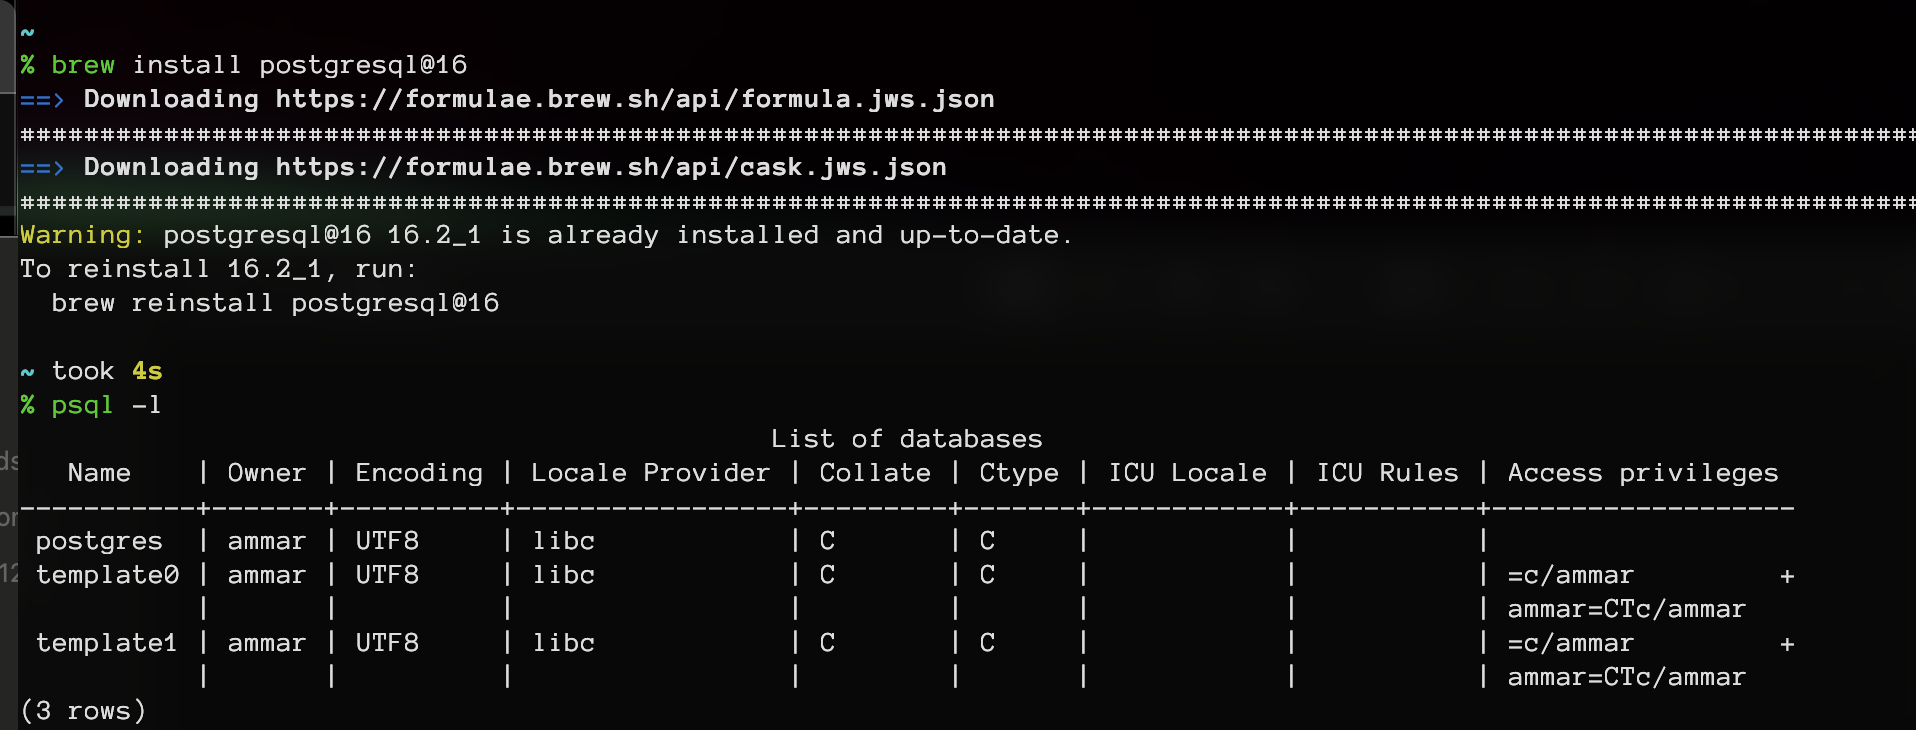
\includegraphics[width=0.6\textwidth]{figures/install_and_list.png}
	\caption{Install PostgreSQL package and checking it works by executing \c{psql -l}, to list all existing databases.}
	\label{fig:install_and_list}
\end{figure}

\section{Startup and Shutdown Options and Procedures} % (fold)
\label{sec:Startup and Shutdown Options and Procedures}
Starting PostgreSQL on Linux/Unix-based systems as in Figure~\ref{fig:Start and stop pgl}.
\begin{figure}[!hb]
	\centering
	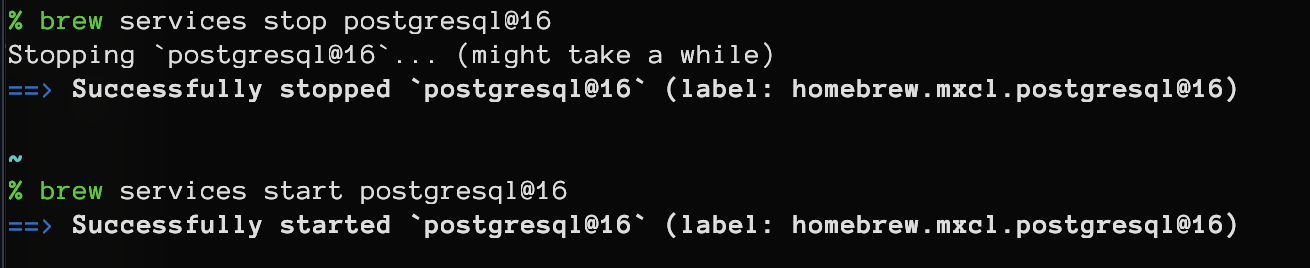
\includegraphics[width=0.6\textwidth]{figures/stop_start_db.png}
	\caption{Start and stop PostgreSQL.}
	\label{fig:Start and stop pgl}
\end{figure}

% section Startup and Shutdown Options and Procedures (end)

\section{Logical and Physical Structures of a Database} % (fold)
\label{sec:Logical and Physical Structures of a Database}
The logical structure of the database is represented by the schema, which defines the tables, relationships, constraints, and other logical entities. The physical structure is how the data is stored on disk, which includes file organization, indexing, and storage parameters.

We can view the logical structure of the Horse database by running the following command:
\begin{lstlisting}
  \d
\end{lstlisting}
See Figure~\ref{fig:list tables} for list of all tables of Horse DB, after I fixed all issues of compatiblity with PostgreSQL-16.
\begin{figure}[!h]
	\centering
	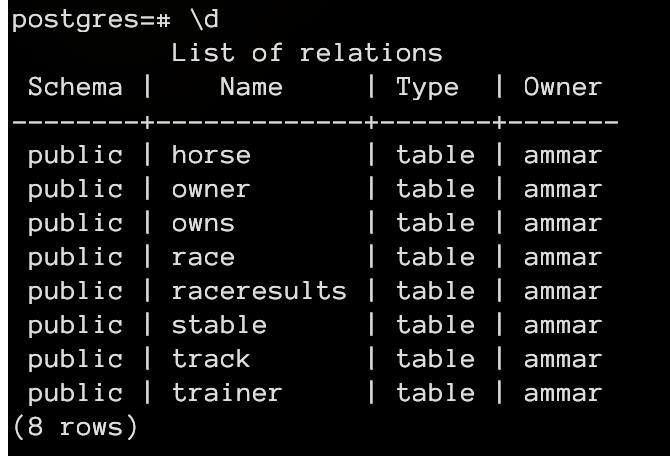
\includegraphics[width=0.3\textwidth]{figures/list_all_tables.png}
	\caption{Listing all tables in the DB.}
	\label{fig:list tables}
\end{figure}

We can also inspect the physical storage parameters using the following command:
\begin{lstlisting}
SELECT relname, relkind, relpages
FROM pg_catalog.pg_class
WHERE relkind IN ('r', 'i', 't');
\end{lstlisting}
This query will display the names of relations (tables, indexes, and toast tables), their type, and the number of disk pages they occupy, see Figure~\ref{fig:index info}.
\begin{figure}[!h]
	\centering
	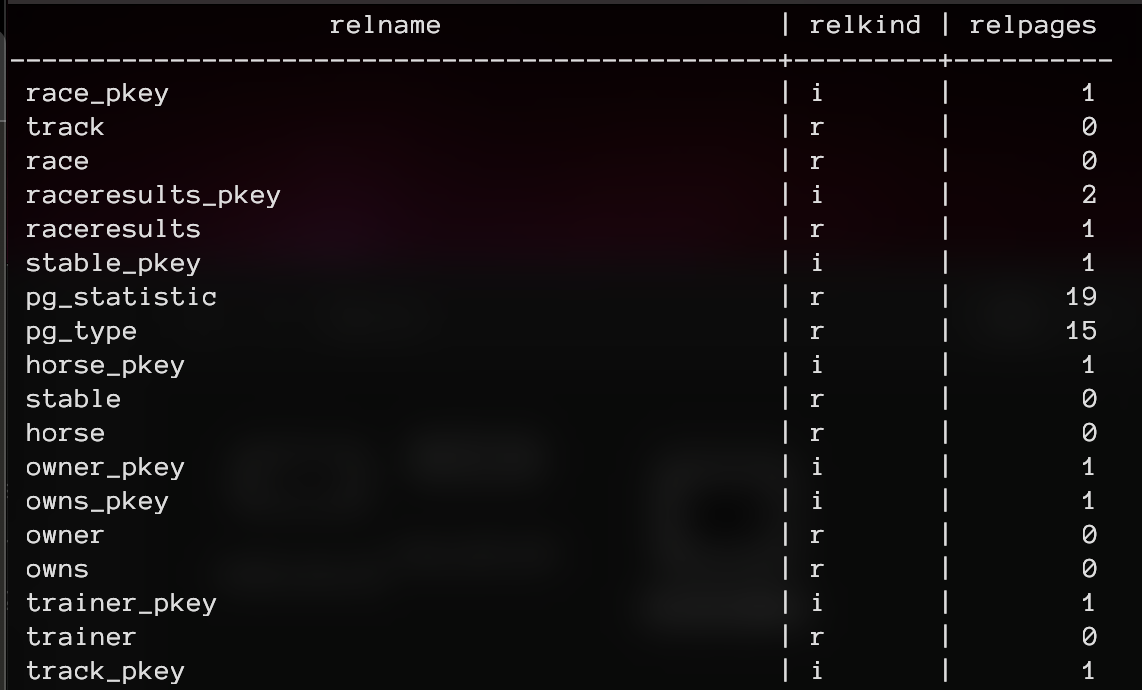
\includegraphics[width=0.3\textwidth]{figures/index_info.png}
	\caption{The names of relations (tables, indexes, and toast tables), their type, and the number of disk pages they occupy.}
	\label{fig:index info}
\end{figure}
% section Logical and Physical Structures of a Database (end)

\section{Creating a Materialized View with a Complex Join} % (fold)
\label{sec:Creating a Materialized View with a Complex Join}
A materialized view is a pre-computed result set that is stored on disk for faster query performance. Here's an example of creating a materialized view that joins multiple tables:
\begin{lstlisting}
CREATE MATERIALIZED VIEW horse_owner_stable_view AS
SELECT h.horseName, o.lname, o.fname, s.stableName, s.location
FROM Horse h
JOIN Owns ow ON h.horseId = ow.horseId
JOIN Owner o ON ow.ownerId = o.ownerId
JOIN Stable s ON h.stableId = s.stableId;
\end{lstlisting}
This materialized view combines data from the Horse, Owns, Owner, and Stable tables to provide a consolidated view of horse names, owner names, and stable information. See Figure~\ref{fig:create view}.
\begin{figure}
	\begin{center}
		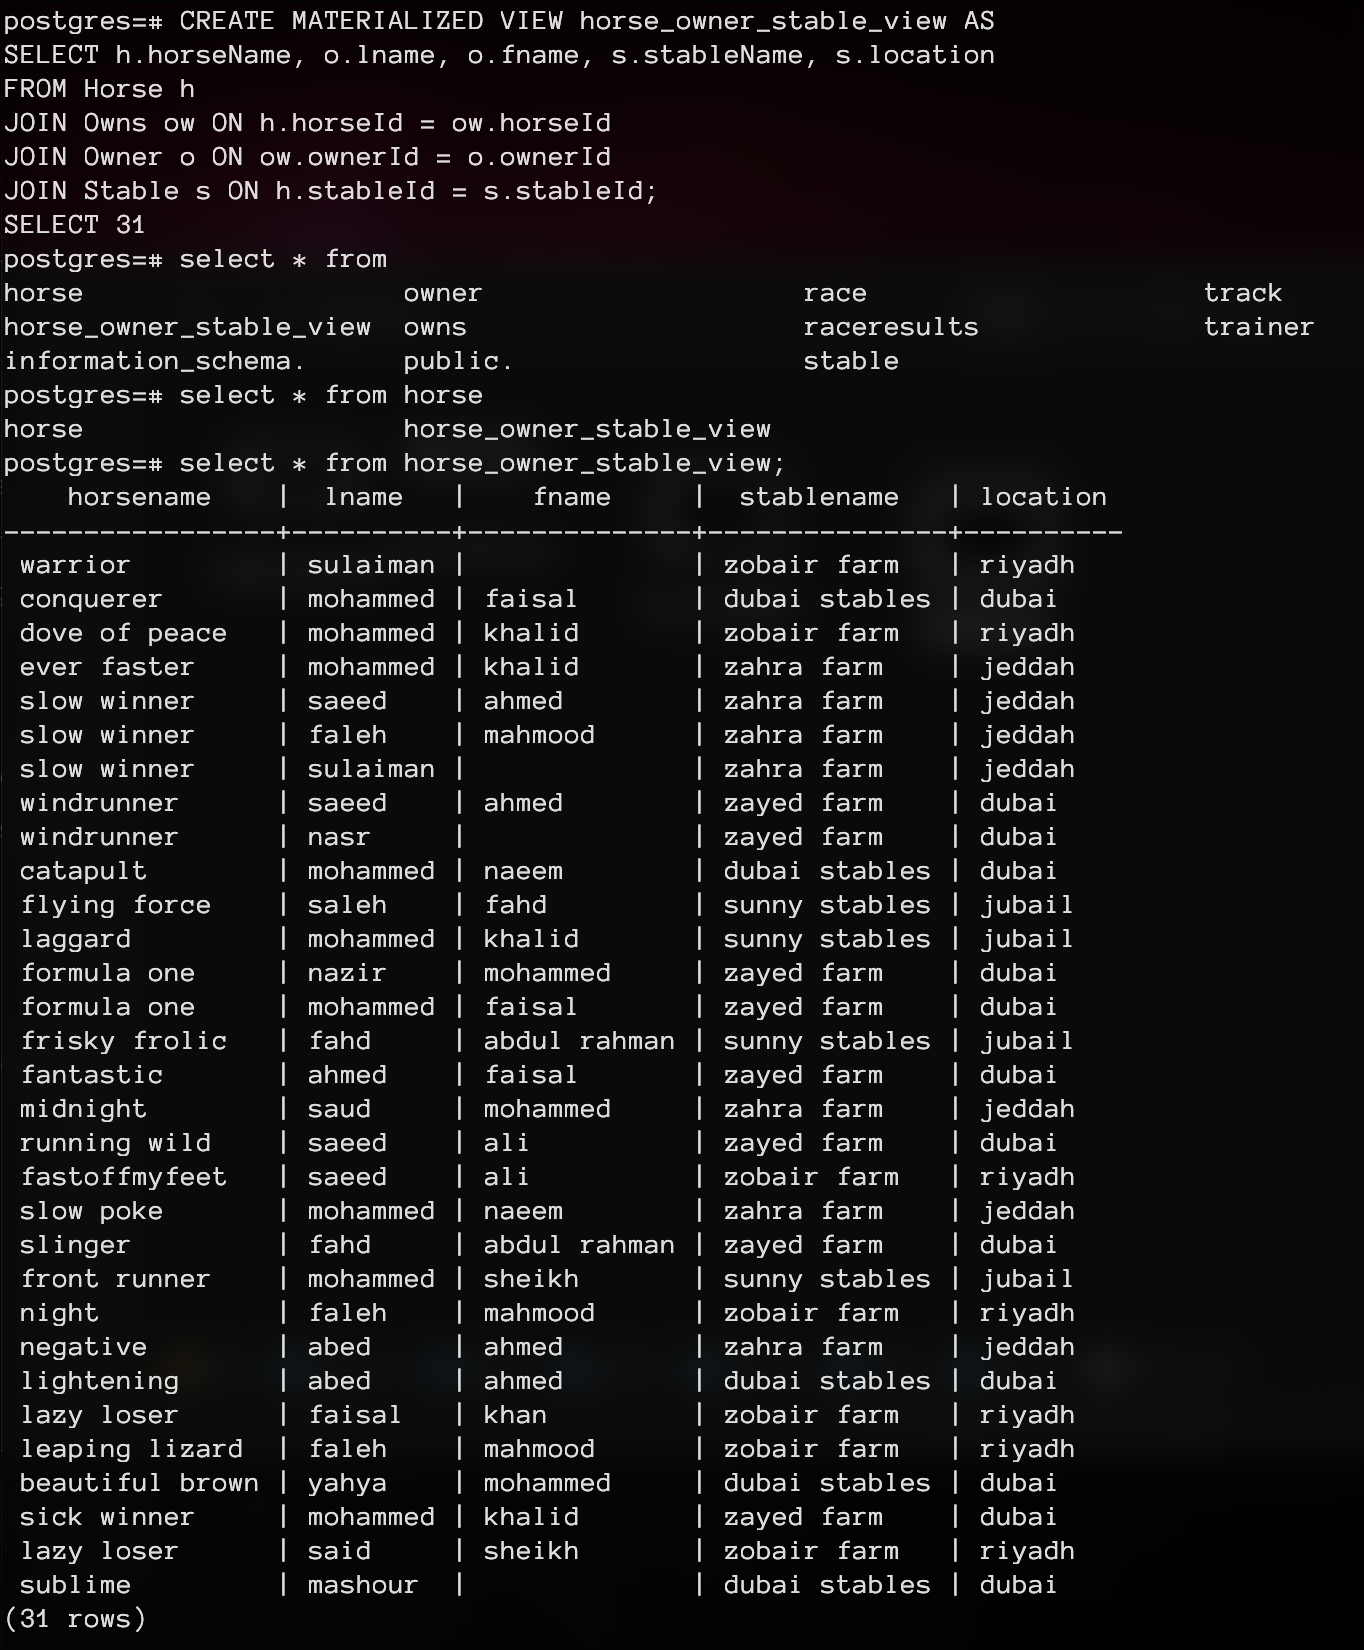
\includegraphics[width=0.5\textwidth]{figures/creating_view.png}
	\end{center}
	\caption{Creating a view and listing all of its contents. }\label{fig:create view}
\end{figure}
% section Creating a Materialized View with a Complex Join (end)

\section{Developing and Demonstrating a Stored Procedure and a Trigger} % (fold)
\label{sec:Developing and Demonstrating a Stored Procedure and a Trigger}
To create a Stored Procedure we run this command:
\begin{lstlisting}
CREATE OR REPLACE FUNCTION update_horse_age()
RETURNS TRIGGER AS $$
BEGIN
    UPDATE Horse
    SET age = age + 1
    WHERE horseId = NEW.horseId;
    RETURN NEW;
END;
$$ LANGUAGE plpgsql;

CREATE TRIGGER update_horse_age_trigger
AFTER INSERT ON RaceResults
FOR EACH ROW
EXECUTE FUNCTION update_horse_age();
\end{lstlisting}
This stored procedure \c{update\_horse\_age()} is triggered after inserting a new row into the RaceResults table. It updates the age of the horse by incrementing it by 1 year. Now, to create a Trigger, we run instead this commmadn:
\begin{lstlisting}
CREATE OR REPLACE FUNCTION prevent_duplicate_owners()
RETURNS TRIGGER AS $$
DECLARE
    owner_count INT;
BEGIN
    SELECT COUNT(*) INTO owner_count
    FROM Owns
    WHERE ownerId = NEW.ownerId AND horseId = NEW.horseId;
    IF owner_count > 0 THEN
        RAISE EXCEPTION 'Owner already owns this horse';
    END IF;
    RETURN NEW;
END;
$$ LANGUAGE plpgsql;

CREATE TRIGGER prevent_duplicate_owners_trigger
BEFORE INSERT ON Owns
FOR EACH ROW
EXECUTE FUNCTION prevent_duplicate_owners();
\end{lstlisting}
This trigger \c{prevent\_duplicate\_owners()} is executed before inserting a new row into the Owns table. It checks if the owner already owns the horse being inserted, and if so, it raises an exception to prevent the insertion.
% section Developing and Demonstrating a Stored Procedure and a Trigger (end)

\section{Demonstrating Locking and Timestamping} % (fold)
\label{sec:Demonstrating Locking and Timestamping}
PostgreSQL provides various locking mechanisms to ensure data integrity and concurrency control. We can observe locking by running two separate sessions and performing conflicting operations. For Session1:
\begin{lstlisting}
BEGIN;
UPDATE Horse SET age = 3 WHERE horseId = 'horse1';
\end{lstlisting}
and for Session2:
\begin{lstlisting}
BEGIN;
UPDATE Horse SET age = 4 WHERE horseId = 'horse1';
\end{lstlisting}
In Session 2, the UPDATE statement will be blocked until Session 1 commits or rolls back its transaction, demonstrating row-level locking. See Figure~\ref{fig:two sessions} for how we can do two transactions.
\begin{figure}
	\begin{center}
		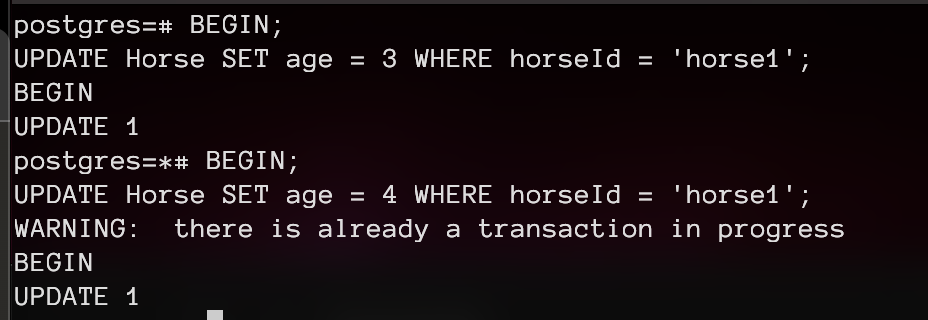
\includegraphics[width=0.5\textwidth]{figures/two_sessions.png}
	\end{center}
	\caption{When we run two sessions we get a warning indicating there's an already running transaction in progress. }\label{fig:two sessions}
\end{figure}


PostgreSQL also supports timestamping to track when data was last modified. We can view the timestamp of a table by running:
\begin{lstlisting}
SELECT xmin, xmax, cmin, cmax, ctid
FROM pg_catalog.pg_class
WHERE relname = 'Horse';
\end{lstlisting}
See Figure~\ref{fig:timestamp table} for the list of existing timestamps.
\begin{figure}
	\begin{center}
		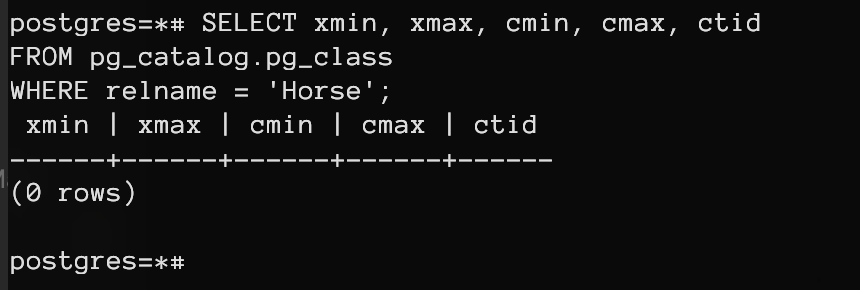
\includegraphics[width=0.5\textwidth]{figures/timestamp_table.png}
	\end{center}
	\caption{Here we see an empty list of the the timestamp table. }\label{fig:timestamp table}
\end{figure}
% section Demonstrating Locking and Timestamping (end)

\section{Diagnosing and Resolving Locking Conflicts} % (fold)
\label{sec:Diagnosing and Resolving Locking Conflicts}
To diagnose locking conflicts, We can use the \c{pg\_locks} view, which provides information about outstanding locks in the database. For example:
\begin{lstlisting}
SELECT l.locktype, l.relation::regclass, l.virtualtransaction, l.pid
FROM pg_locks l
JOIN pg_stat_activity a ON l.pid = a.pid;
\end{lstlisting}
This query displays the lock type, relation (table) name, virtual transaction ID, and process ID of the locks, as seen in Figure~\ref{fig:pg_lock}.
\begin{figure}
	\begin{center}
		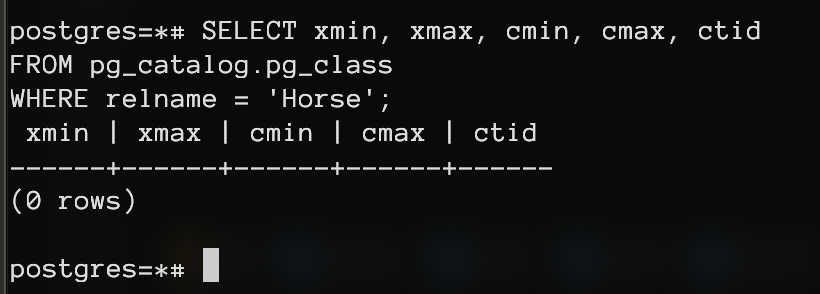
\includegraphics[width=0.5\textwidth]{figures/pg_lock.png}
	\end{center}
	\caption{PostgreSQL lock table}\label{fig:pg_lock}
\end{figure}

To resolve locking conflicts, we can either wait for the blocking transaction to complete or terminate the blocking process using the \c{pg\_terminate\_backend()} function. See Figure~\ref{fig:terminate pid} for how we can terminate processes from their PID.
\begin{figure}
	\begin{center}
		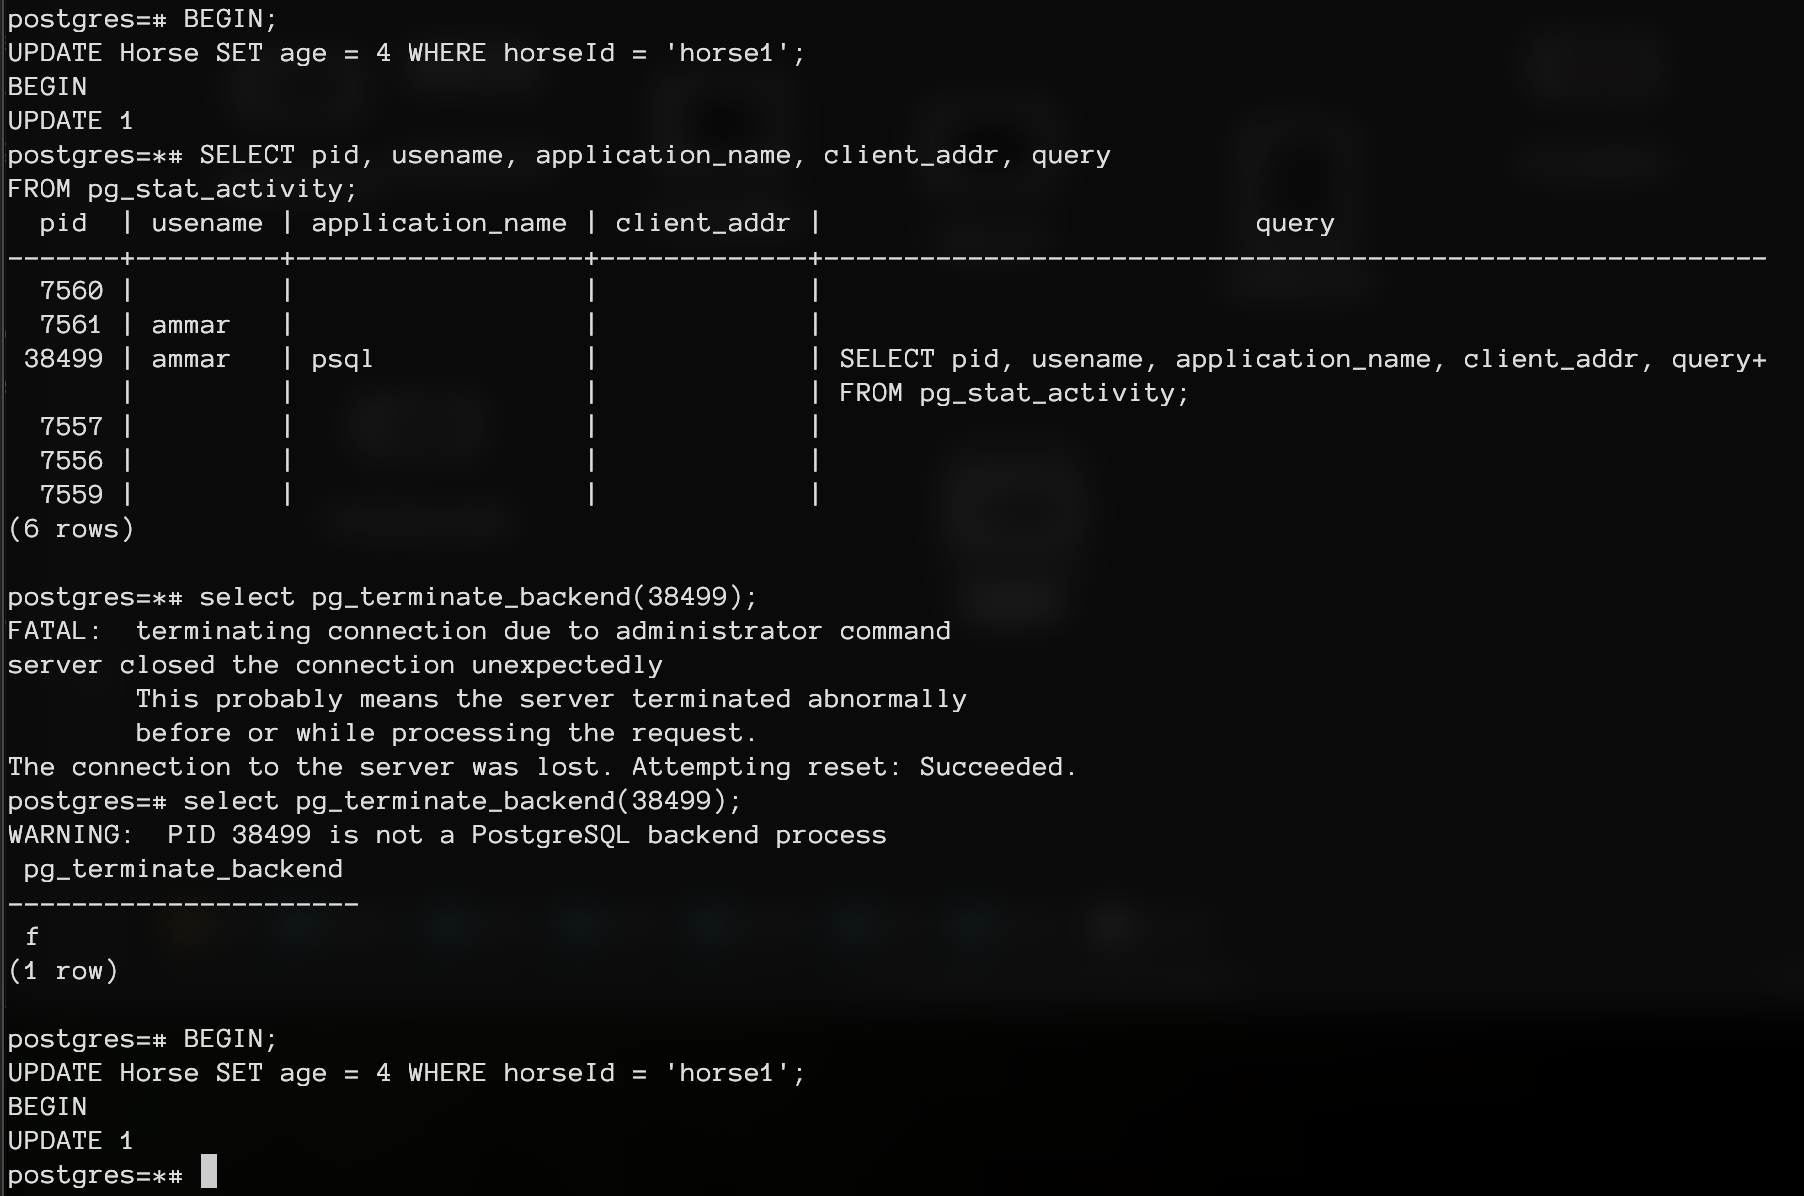
\includegraphics[width=0.5\textwidth]{figures/terminating_pid.png}
	\end{center}
	\caption{We searched up for a running process's PID and then terminate it.}\label{fig:terminate pid}
\end{figure}
% section Diagnosing and Resolving Locking Conflicts (end)

\section{Evaluating Backup Options} % (fold)
\label{sec:Evaluating Backup Options}
PostgreSQL offers several backup options, including:

\begin{itemize}
	\item \textbf{SQL Dump:} This creates a plain-text file containing SQL statements to recreate the database objects and data. We can create a SQL dump using the \c{pg\_dump} utility.
	\item \textbf{File System Level Backup:} This involves creating a consistent backup of the PostgreSQL data directory using file system-level tools like tar or disk-level backup utilities.
	\item \textbf{Continuous Archiving and Point-in-Time Recovery (PITR):} This technique involves archiving Write-Ahead Log (WAL) segments, which can be used to restore the database to a specific point in time.
\end{itemize}
We can evaluate and choose the appropraite backup option based on our requirements, such as backup size, restore time, and the need for point-in-time recovery.
% section Evaluating Backup Options (end)

\section{Recovering a Database} % (fold)
\label{sec:Recovering a Database}
To recover a database from a backup, follow these general steps:
\begin{enumerate}
	\item Stop the PostgreSQL server.
	\item Replace the data directory with the backup files (for file system level backup) or restore the SQL dump (for SQL dump backup).
	\item Start the PostgreSQL server.
	\item If using PITR, restore the database from the archived WAL segments to the desired point in time.
\end{enumerate}
% section Recovering a Database (end)

\section{Creating and Managing Indexes} % (fold)
\label{sec:Creating and Managing Indexes}
Indexes improve query performance by allowing faster data retrieval. To create an index on a table column, use the CREATE INDEX statement:
\begin{lstlisting}
CREATE INDEX idx_horse_age ON Horse (age);
\end{lstlisting}
This creates an index named \c{idx\_horse\_age} on the age column of the Horse table.

We can view existing indexes using the following query:
\begin{lstlisting}
SELECT relname, relkind, indkey
FROM pg_catalog.pg_index
JOIN pg_catalog.pg_class ON pg_index.indexrelid = pg_class.oid
WHERE relname LIKE 'idx_%';
\end{lstlisting}

To drop an index, use the DROP INDEX statement:
\begin{lstlisting}
DROP INDEX idx_horse_age;
\end{lstlisting}
See Figure~\ref{fig:create idx}, how apply all above in the \c{age} column in \c{Horse} table.
\begin{figure}
	\begin{center}
		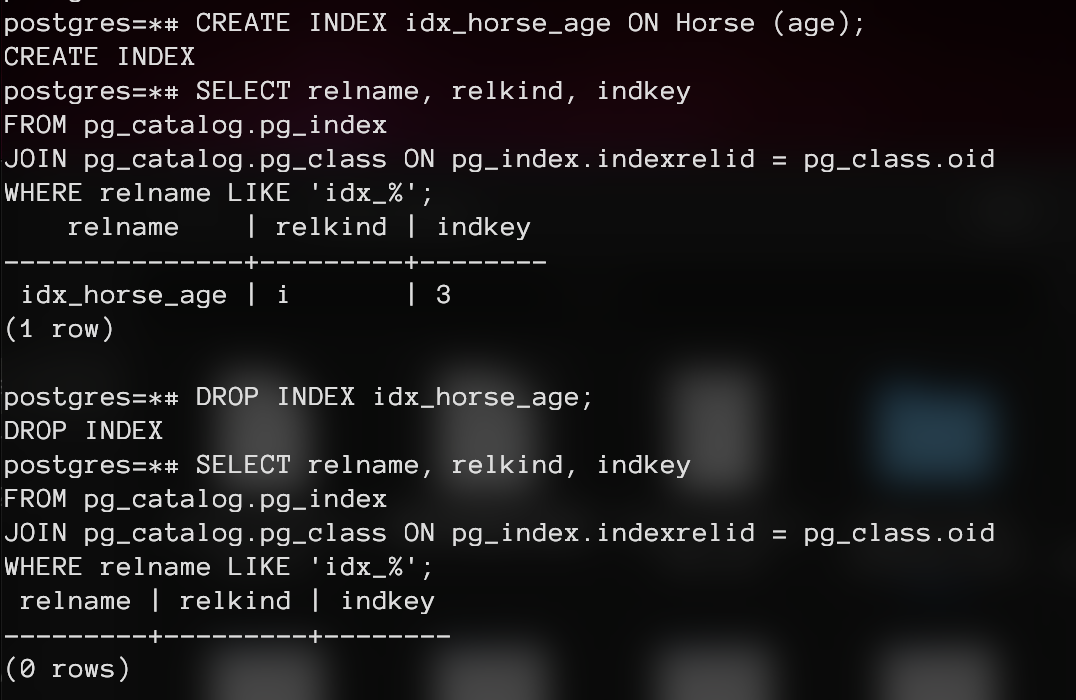
\includegraphics[width=0.5\textwidth]{figures/create_drop_idx.png}
	\end{center}
	\caption{We created an index on \c{age} column, view it, and drop at the end as demonstration.}\label{fig:create idx}
\end{figure}
% section Creating and Managing Indexes (end)

\section{Collecting and Analyzing Database Performance Information} % (fold)
\label{sec:Collecting and Analyzing Database Performance Information}
PostgreSQL provides several tools and views for collecting and analyzing performance information, such as:
\begin{itemize}
	\item \c{pg\_stata\_user\_tables}: This view provides statistical information about tables, including the number of rows, disk space usage, and the last autovacuum and autoanalyze times.
	\item \c{pg\_stat\_user\_indexes}: This view provides statistical information about indexes, including the number of index scans and the index size.
	\item \c{pg\_stat\_database}: This view provides statistics about database-level activity, such as the number of transactions, tuples read and written, and blocks read and written.
	\item \c{EXPLAIN} and \c{EXPLAIN ANALYZE}: These commands provide execution plans for SQL queries, including the estimated and actual costs, and information about the operations performed.
\end{itemize}
We can use these tools to analyze query performance, identify bottlenecks, and optimize our database for better efficiency.

Here's an example of using EXPLAIN ANALYZE to analyze the performance of a query:
\begin{lstlisting}
EXPLAIN ANALYZE
SELECT h.horseName, o.lname, o.fname
FROM Horse h
JOIN Owns ow ON h.horseId = ow.horseId
JOIN Owner o ON ow.ownerId = o.ownerId
WHERE h.age > 3;
\end{lstlisting} \label{lst:exec plan}
This will display the execution plan for the query, including the actual time and cost for each operation, providing insights into potential performance bottlenecks. See Figure~\ref{fig:exec plan}, for the analysis of execution plan for the Listing~\ref{lst:exec plan}.

\begin{figure}
	\begin{center}
		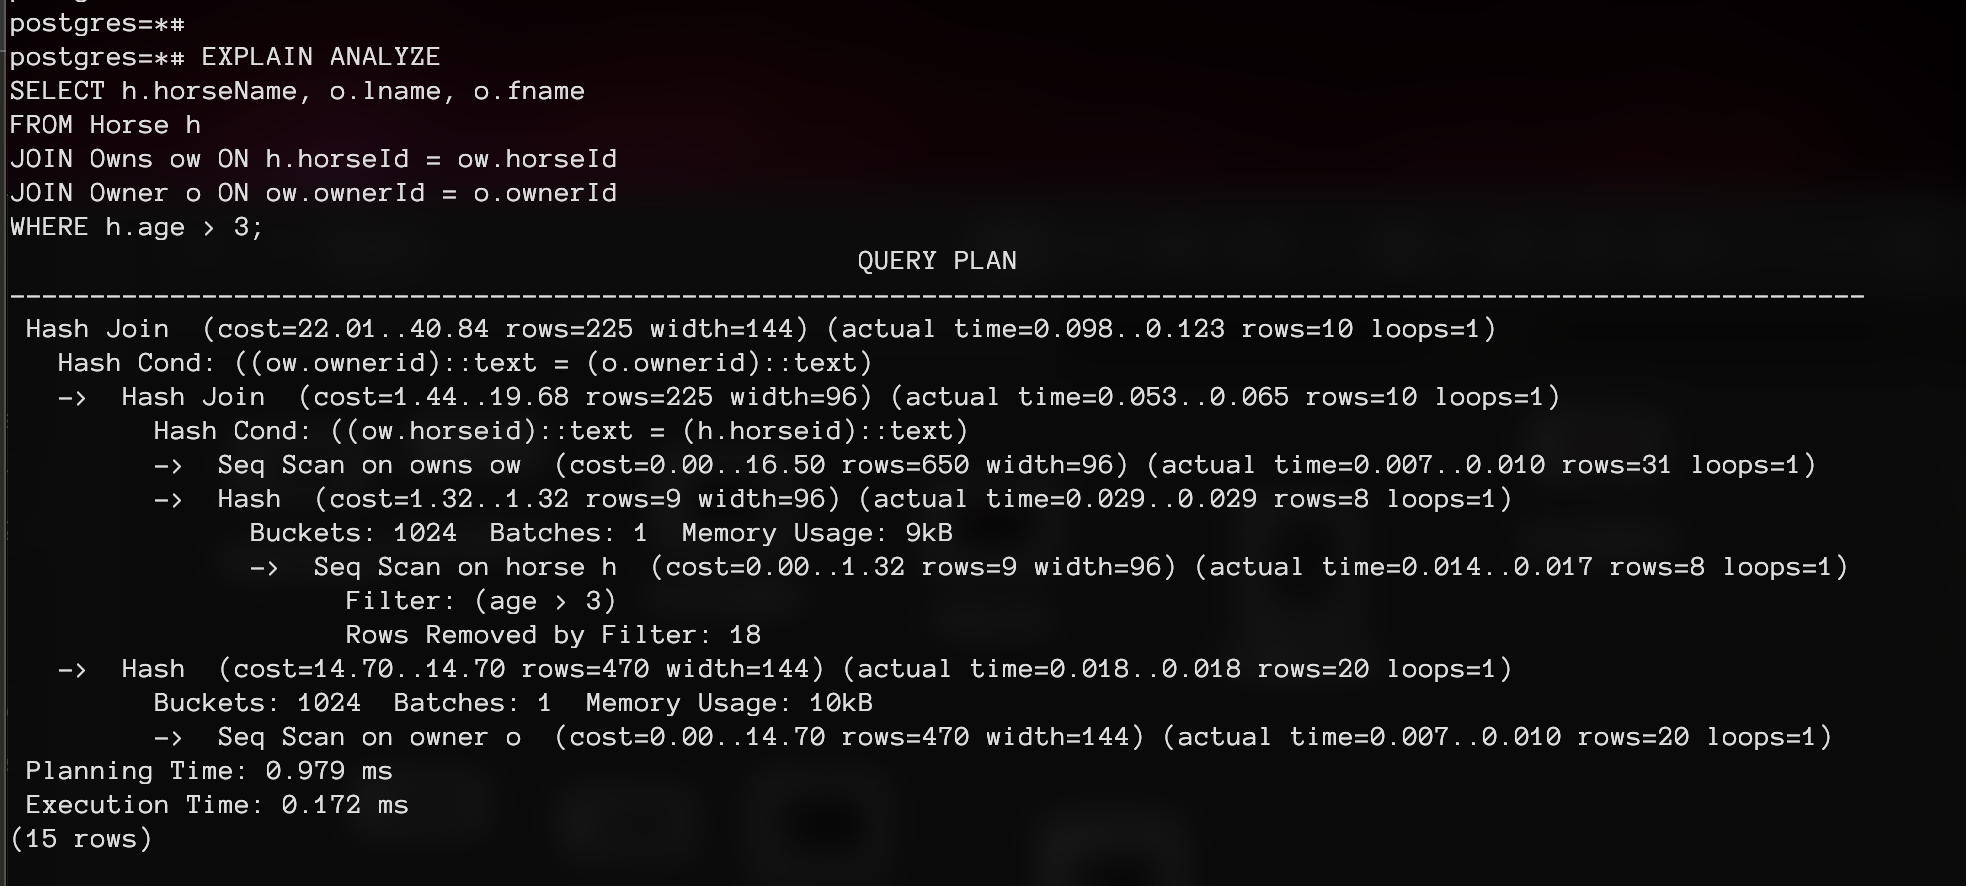
\includegraphics[width=0.95\textwidth]{figures/exec_plan.png}
	\end{center}
	\caption{An execution plan example.}\label{fig:exec plan}
\end{figure}
% section Collecting and Analyzing Database Performance Information (end)

\end{document}
